\chapter{Analiza problemu}
\thispagestyle{chapterBeginStyle}
\label{rozdzial1}
W niniejszym rozdziale omówiono problem redundancji oraz powiązanych pojęć, czyli detekcji i korekcji błędów. Opisano rownież zastosowane rozwiązania w ogólnym modelu systemu oraz relacje pomiędzy komponentami pracy, które wykorzystano w celu osiągnięcia jak największej niezawodności danych.

Implementowany projekt należy do grupy wirtualnych systemów plików, co pozwala na łatwe oraz intuincyjne montowanie w dowolnym miejscu dla wybranych katalogów, przez co w różnych miejscach nadrzędnego systemu plików mogą być zamontowane różne metody redundancji danych. Możliwe jest również wykorzystanie różnych nośników danych. 

Struktura systemu w założeniu jest rozłożona na warstwy. To znaczy, że każda opisywana funkcjonalność jak kodowanie czy odzyskiwanie plików jest niezależna od pozostałych i działają bez znajomości poprzedzających warstw. Takie rozwiązanie ułatwia dodawanie kolejnych funkcjonalności, czy rozszerzanie obecnych o nowe implementacje.

Założenia omawianego systemu:
\begin{itemize}
    \item Obsługa różnych rozwiązań redundancji
    \item Obsługa wielu kopii plików w celu zwiększenia niezawodności danych
    \item Wybór najodpowiedniejszej repliki do odczytu pliku 
    \item Synchronizacja już stniejących plików pomiędzy kopiami
	\item Obsługa przynajmniej podstawowych zachowań systemu plików:
		\begin{itemize}
			\item Czytanie oraz pisanie do plików
			\item Tworzenie oraz usuwanie plików
		\end{itemize}
	\item Detekcja błędów:
		\begin{itemize}
			\item Walidacja poprawności danych w pliku podczas odczytu
			\item Walidacja poprawności plików między kopiami 
		\end{itemize}
	\item Korekcja błędów:
		\begin{itemize}
			\item Zastosowanie kodów korekcyjnych
			\item Całkowite zastępowanie uszkodzonych plików poprawnymi kopiami
		\end{itemize}
    \item Wygoda użytkowania
\end{itemize}

\section{System plików}
Do implementacji systemu plików wykorzystano interfejs FUSE, moduł w Unixowych jądrach pozwalający na tworzenie systemu plików w przestrzeni użytkownika. To rozwiązanie pozwala skupić się na tworzeniu pożądanej funkcjonalności, bez potrzeby schodzenia do poziomu jądra systemu. Projekt został zbudowany jako wirtualny system plików. Skupia się na translacji danych które otrzymuje, resztą zajmuje się nadrzędny system plików oraz moduł FUSE. 

\section {Redundancja danych}
Nadmiarowość zapisywanych informacji jest często stosowana w celu wykrycia uszkodzonych danych lub zabezpieczenia ich przed utratą po częściowym, czy całkowitym uszkodzeniu.
Redundancja danych stanowi najwazniejsze zagadnienie rozwazanej pracy. Zaproponowano kilka roznych rozwiazan, aby przedstawic zakres mozliwosci systemu. Rozwiazania oparte sa na macierzy RAID ze wzgledu na ich skutecznosc oraz mozliwosc tworzenia kombinacji standardowych poziomow.

\subsection {RAID}
Redundant Array of Independent Disks to metoda wirtualizacji przechowywania danych. Wykorzystuje wiele dyskow i laczy je w logiczne jednostki pamieci. RAID jest stosowane do redundancji danych oraz lepszej wydajnosci, jednak w niniejszej pracy wydajnosc systemu nie bedzie rozwazana.  
RAID jest zbiorem schematow rozwiazan, ktore nazywane sa poziomami. Na potrzeby pracy przedstawione zostana wybrane poziomy, ktore wprowadzaja rozne metody redundancji.
\subsubsection{Poziom 0}
RAID-0 jako jedyny poziom RAID wprowadza zerowa redundancje. Laczy przynajmniej dwa fizyczne nosniki danych w jeden dysk logiczny i w tej przestrzeni przeplata dane pomiedzy dyskami. Dane sa dzielone na bloki o stalym rozmiarze. Poziom 0 w zaden sposob nie zapewnia niezawodnosci danych, jednak stanowi podstawe do innych poziomow. Wykorzystanie przeplotu danych na wiele dyskow usprawnia operacje odczytu i zapisu wykonujac je rownolegle na wszystkich dyskach macierzy.
\begin{figure}[h!]
        \centering
        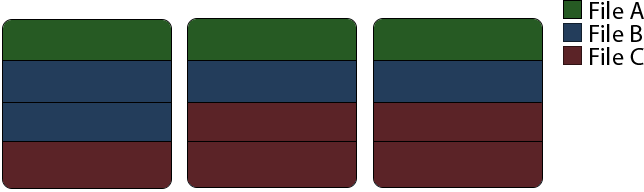
\includegraphics[scale=0.8]{raid-0.png}
        \caption{RAID-0 z trzema dyskami}
        \label{fig:raid0}
\end{figure}
\newpage
\subsubsection{Poziom 1}
RAID-1 dziala na przynajmniej dwoch dyskach. Dane sa zapisywane do wszystkich dyskow, tworzac lustrzane odbicia. Z tego wzgledu czas wykonywania dowolnych operacji jest rowny sumie czasu trwania danej operacji na wszystkich dyskach, jednak mozliwe jest przyspieszenie dzialania. RAID-1 chroni przed utrata $(n-1)$ dyskow macierzy, jednak przez to wymaga duzej ilosci miejsca; dla $n$ dyskow o rozmiarze $m$ potrzebne jest $n\times m$ wolnej przestrzeni.
\begin{figure}[h!]
        \centering
        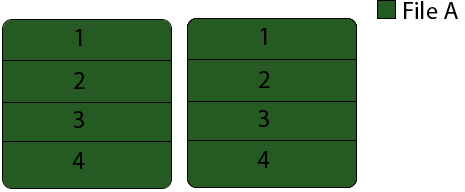
\includegraphics[scale=0.8]{raid-1.png}
        \caption{RAID-1 z dwoma dyskami}
        \label{fig:raid1}
\end{figure}
\subsubsection{Poziom 2}
Podobnie do RAID-0, dane sa dzielone miedzy dyskami. W przypadku poziomu drugiego, dane sa dzielone na pojedyncze bity, a kazdy bit jest zapisywany na kolejnym dysku. RAID-2 wykorzystuje kod Hamminga do korekcji wystepujacych bledow, wszystkie bity kodu znajduja sie w odpowiednich dyskach i  pozwalaja na odzyskanie danych z jednego uszkodzonego dysku. 
\begin{figure}[h!tb]
        \centering
        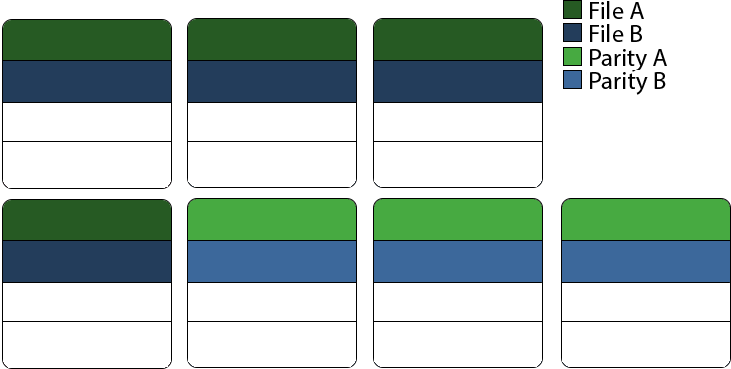
\includegraphics[scale=0.8]{raid-2.png}
        \caption{RAID-2 na siedmiu dyskach}
        \label{fig:raid2}
\end{figure}
\subsubsection{Poziom 4}
Dane sa dzielone na bloki ograniczonej wielkosci i tak jak w przypadku poziomu 0, kazdy blok jest zapisywany na kolejnym dysku. Do przechowywania danych sluzy $n-1$ dyskow. Dla kazdego rzedu zapisanych danych obliczany jest blok parzystosci na osobnym dysku. Po uszkodzeniu jednego z dyskow pojedynczy blok moze zostac odzyskany.
\begin{figure}[h!]
        \centering
        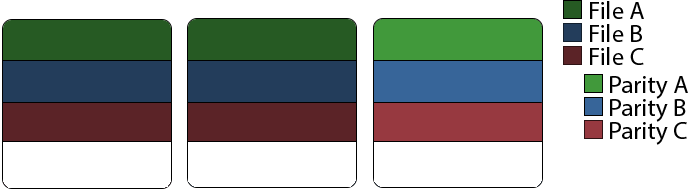
\includegraphics[scale=0.8]{raid-4.png}
        \caption{RAID-4 na trzech dyskach}
        \label{fig:raid4}
\end{figure}
\subsubsection{Poziom 5}
Dane sa dzielone i bity parzystosci sa obliczane podobnie do poprzedniego poziomu, jednak bloki parzystosci obliczane z $n-1$ blokow danych nie sa zapisywane na dedykowanym dysku, tylko rozkladane rownomiernie na wszystkich dyskach macierzy. Stad dostepna pojemnosc to rowniez $n-1$ i mozliwe jest odzyskanie jednego uszkodzonego dysku.
\begin{figure}[h!]
        \centering
        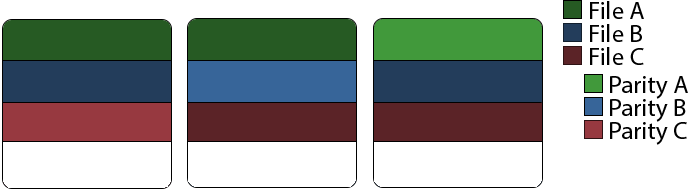
\includegraphics[scale=0.8]{raid-5.png}
        \caption{RAID-5 na trzech dyskach}
        \label{fig:raid5}
\end{figure}
\subsubsection{Poziom 6}
t
\newpage
\subsection{Standardowe repliki systemu}
Repliki zostaly zaprojektowane na podstawie poziomow RAID. Roznia sie miedzy soba sposobem wprowadzenia redundancji danych oraz mozliwym zastosowaniem. System funkcjonuje z jedna replika, kosztem nizszej redundancji. Ponizej opisano proponowane rodzaje replik oraz rozwazono ich mocne i slabe strony. Wszystkie rodzaje mozna podzielic na dwie kategorie:
\begin{itemize}
    \item Replika standardowa - Dokonuje detekcji bledow w plikach, jednak w przypadku wykrycia takiego bledu lub desynchronizacji z innymi replikami, nie jest w stanie dokonac korekty bledow bez dodatkowych replik
    \item Replika korekcyjna - Dokonuje zarowno detekcji, jak i korekcji znalezionych bledow. Jesli korekta znalezionych bledow jest niemozliwa, zachowuje sie podobnie do repliki bez korekty - desynchronizacja moze zostac naprawiona wylacznia z dodatkowymi replikami
\end{itemize}
Repliki korekcyjne dodają funkcjonalność do standardowej, dlatego zostały omówione w późniejszej sekcji pracy. 

W przypadku trwałej awarii repliki takiej jak uszkodzenie dysku, replika zostaje oznaczona jako nieaktywna i nie są podejmowane kolejne próby odczytu czy zapisu danych.
\subsubsection{Repliki Lustrzane (MR)}
Oparte na schemacie RAID-1 repliki tego typu stanowią lustrzane odbicie danych. Każdy plik występuje dokładnie raz we wszystkich replikach lustrzanych.
\begin{itemize}
        \item Naprawia błędy innych replik kopiując całe pliki
        \item Wszystkie dane zamontowane w jednym miejscu. W przypadku, kiedy jeden dysk zostanie uszkodzony, dane zostają utracone.
\end{itemize}

\begin{figure}[h!]
        \centering
        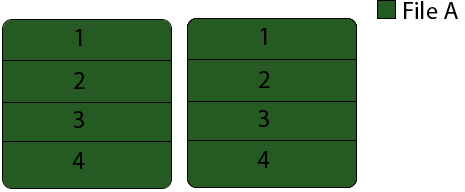
\includegraphics{raid-1.png}
        \caption{Dwie repliki lustrzane}
        \label{fig:raid1}
\end{figure}

Standardowe MR nie są w stanie naprawić uszkodzonych plików. Jedynym rozwiązaniem jest zastąpić uszkodzone pliki w całości danymi z innej repliki. Repliki lustrzane z korektą błędów opisane w dalszej części pracy rozszerzają funkcjonalność podstawowych replik.
\subsubsection{Repliki Blokowe (BR)}
W replikach tego typu pliki są rozkładane na części i zapisywane w kolejnych katalogach będących odpowiednikiem dysków poziomu RAID-0. Tak samo katalogi mogą być rozmieszczone na różnych urządzeniach przechowujących. Każdy z katalogów może również być repliką. Jedna część pliku nazywana jest dalej blokiem.
Rozkład danych jest możliwy na dwa sposoby:
\begin{itemize}
    \item Pliki podzielone na stałą ilość bloków. 

            Zmiana wielkości pliku może powodować zmianę rozmiaru wszystkich bloków danego pliku dla wyrównania wielkości, lub jedynie tego bloku, do którego dane zostają dopisane. W takim wypadku bloki nie są jednakowych rozmiarów. Możliwe jest ograniczenie rozmiaru pojedynczego bloku, tym samym ograniczając maksymalny rozmiar pliku.
            \begin{figure}[h!]
                    \centering
                    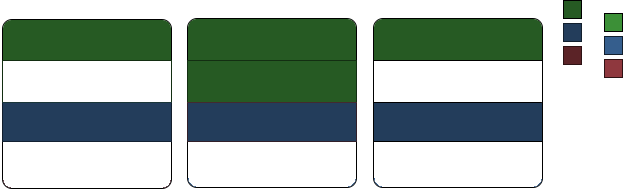
\includegraphics{BR-1.png}
                    \caption{Podział pliku na trzy nierówne bloki }
                    \label{fig:br1}
            \end{figure}
    \item Pliki podzielone na zmienną ilość części o ograniczonych wielkościach

            Określony jest maksymalny dozwolony rozmiar dla pojedynczego bloku. Przy przekroczeniu rozmiaru bloku, system tworzy kolejny w następnym katalogu dopóki jest miejsce. 
            \begin{figure}[h!]
                    \centering
                    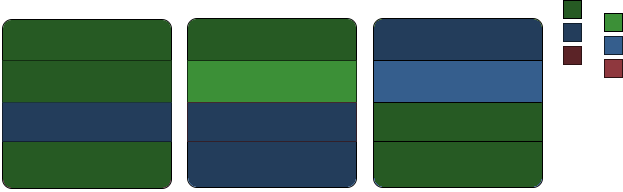
\includegraphics{BR-2.png}
                    \caption{Podzial pliku na wiele bloków ograniczonego rozmiaru}
                    \label{fig:br1}
            \end{figure}
 
\end{itemize}
Standardowe repliki blokowe nie są w stanie naprawić uszkodzonych plików, jednak taki podział danych wpłynie korzystnie na repliki korekcyjne i jest szczególnie przydatny dla wielu dysków. Jeśli replika blokowa działa na $n$ blokach, działa również po awarii na $n-1$ dyskach dla $n < 1$. Dodatkowo, replika blokowa rozszerzona o korekcję danych, może odzyskać utracony blok danych.

W przypadku awarii jednego z bloków repliki, replika jest nadal aktywna wtedy i tylko wtedy, jeśli odzyskano utracone dane i replika jest nadal w pełni funkcjonalna. Jeśli awarii uległ ostatni blok, a system nie może ustalowić nowej lokalizacji dla przynajmniej jednego bloku, replika zostaje uznana za nieaktywną.
\begin{itemize}
    \item Naprawia błędy innych replik kopiując jedynie częściowe pliki, jeśli to możliwe.
    \item Dane mogą zostać zamontowane w wielu miejscach. W przypadku uszkodzenia jednego dysku, reszta danych jest nadal dostępna.
\end{itemize}

\subsection{Podzial replik na warstwy}
W celu ulatwienia rozszerzalnosci dzialania replik, kolejne funkcjonalnosci skladaja sie na niezalezne warstwy. W przypadku, kiedy uzytkownik chce dodac nowe funkcje lub zmienic obecne, powinien byc w stanie to zrobic bez koniecznosci zmian w niepowiazanych czesciach systemu.


\section {Detekcja błędów}
    Wykrywanie bledow ma kluczowe znaczenie w dzialaniu opisywanego systemu. Po znalezieniu bledow plikow, moze nastapic proba naprawienia badz zastapienia uszkodzonych danych bez potrzeby ingerencji uzytkownika. Wszystkie techniki detekcji bledow dodaja kolejne bity do zapisu, tym samym zwiekszajac redundancje w systemie. Korzystanie z kontroli bledow niesie za soba wykonywanie dodatkowych obliczen nawet podczas wykonywania podstawowych operacji na plikach, za kazdym razem sprawdzajac poprawnosc danych. Kazda metoda ma kilka roznych rozkladow danych wynikajacych ze struktury replik. Niektore metody detekcji przy odpowiednich warunkach moga od razu dokonywac korekty wykrytych bledow, co zostalo dokladniej opisane w kolejnym punkcie.
\subsection{Kod Hamminga}
Kod Hamminga jest kodem korekcyjnym, wykrywa i naprawia błędy pojedynczego bitu. Chociaż szczegóły części korekcji zostają omówione w dalszej części pracy, kod Hamminga zostaje również wykorzystany do samej detekcji błędów dwóch bitów.
Odległość Hamminga $H_D$ mierzy liczbę miejsc, w których dwa ciągi o tej samej długości różnią się od siebie. Minimalna odległóść Hamminga dla kodu to najmniejsza odległość pomiędzy dowolnymi dwoma słowami z kodu. Dla kodów określa dwie ważne dla opisywanego problemu własności:
\begin{itemize}
        \item Kod  o minimalnej odległości $H_D = d$ może wykryć $(d-1)$ błędów
        \item Kod o minimalnej odległości $H_D = d$ może naprawić $floor\left(\dfrac{(d-1)}{2}\right)$ błędów
\end{itemize}
Kody Hamminga mają określony minimalną odległość $H_D = 3$, więc z powyższych własności są w stanie wykrywać błędy do dwóch bitów.  W implementowanym systemie, kod Hamminga został wykorzystany zarówno jako metoda korekcji pojedynczego błędu w blokach określonego rozmiaru, jak i detekcji dwóch błędów.


\subsection{Sumy kontrolne}
    W celu weryfikacji, czy dane znajdujące się w pliku nie uległy niepożądanej zmianie, operacje wpływające na zawartość pliku obliczają sumę kontrolną. Niezgodność sumy zapisanej z wyliczoną podczas próby odczytu oznacza wystąpienie błędu w danych pliku lub w samej sumie kontrolnej. Sumy kontrolne zapewniaja spojnosc danych i sa dołączane na koniec sprawdzanych danych, lub jako osobny plik. 
\subsubsection{Funkcje skrotu}
Funkcje skrotu sa wykorzystywane do tworzenia krotkich, latwych do zweryfikowania, podpisow. Obliczone sygnatury sa dolaczane do danych i chronia przed nieautoryzowanymi modyfikacjami danych. Funkcje skrotu zwracaja kod stalego rozmiaru dla zbioru danych o dowolnej wielkosci. Funkcja przechodzi ze zbioru ciagow dowolnej dlugosci do zbioru kodow o stalej dlugosci, wiec moze dojsc do kolizji. Kolizja wystepuje kiedy dla dwoch roznych od siebie slow kodowanych funkcja zwraca te sama wartosc, uniemozliwiajac wykrycie zmiany w zapisanych danych. Funkcja MD5 zostala wybrana do obliczania sygnatur plikow.
\subsubsection{Kontrola parzystosci}
Do zapisywanych danych mozna dopisac dodatkowe informacje o parzystosci ustawionych bitow. Niech slowo kodowane $x \in (0,1)^n$ dla pewnego $n \ge 1$. Wtedy mozliwe jest obliczenie $x_p = x_1 \oplus x_2 \oplus \cdots \oplus x_k$ dla $x_i$ takich, ze $x_i = 1$. $x_p = 0$ jesli ilosc jedynek jest parzysta, $x_p$ w przeciwnym wypadku. 

Niepozadana zmiana nieparzystej ilosci bitow zostanie wykryta, poniewaz funkcja $xor$ przybierze wartosc przeciwna poprzedniej. Zmiany parzystej ilosci bitow pozostana niezauwazane.

\section {Korekcja błędów}
Kodowanie korekcyjne umozliwia wykrywanie i korygowanie okreslonych bledow. Kod korekcyjny jest zapisywany w formie redundantnej wraz z danymi, kodujac wartosci bitow podczas zapisu. W przypadku wystapienia złych bitów podczas odczytu, kody korekcyjne mogą spróbować naprawić znalezione błędy bez wiedzy użytkownika.
\subsection{Kod Hamminga}
Wykorzystanie Kodu Hamminga zostałe opisane, jednak przy korekcji błędów należy rozważyć pewną własność. Chociaż kodowanie pozwala na wykrycie dwóch błędów, w żaden sposób nie odróżnia błędów jednego bitu słowa od dwóch bitów. Z tego wynika, że jeśli system zawsze podejmie się próby korekcji słowa kodowanego po wykryciu błędu, słowo w niektórych przypadkach może zostać źle naprawione.
Dla zwiększenia skuteczności kodowanie, do kodu zostaje dodany dodatkowy bit parzystości. Kodowanie Hamminga z bitem parzystości zwiększa minimalną odległość $H_D$ = 4, co pozwala deterministycznie rozpoznać, czy znaleziono błąd jednego, czy dwóch bitów. Co więcej, jeśli kod Hamminga jest wykorzystywany jedynie do detekcji błędów, odległóść $H_D$ o wartości 4 oznacza, że dekoder może niezawodnie wykryć do trzech błędów.  
\subsection{Kodowanie Reeda-Solomona}
TODO
\subsection{Parzystość}
Kontrola parzystosci pozwala odzyskac wartosc pojedynczego bitu danych. Jesli wartosc pojedynczego bitu zostala utracona, informacja o ilosci ustawionych bitow w kodowanym ciagu wystarcza, aby rozpoznac wartosc brakujacego bitu.  
\subsection{Repliki korekcyjne}
Dodanie metod korekcji błędów w replikach blokowych umożliwi odzyskiwanie całych bloków. Jeśli utracony blok posiadał jedynie kodowane dane, to traktując brakujący blok repliki jako zerowe bity, rozwiązania takie jak bity parzystości posiadają dostatecznie dużo informacji na temat danych, aby wyliczyć brakujące informacje. W takim wypadku repliki mogą zmienić lokalizację odzyskanego bloku danych lub dzielić dane na mniejszą ilość bloków. 

Ważny jest rozkład danych przy dodatkowej redundancji wynikającej z dodania do słów obliczonych kodów. W przypadku replik lustrzanych, możliwe są dwa rozwiązania:
\begin{itemize}
        \item Zapisywanie bitów kodu na końcu pliku
        \item Zapisywanie bitów kodu razem z kodowanymi danymi
\end{itemize}
Dla replik blokowych, ze względu na ich rozproszoną strukturę, przedstawiono następujące możliwości:
\begin{itemize}
        \item Zapisywanie bitów kodu bitów osobno od kodowanych danych na jednej replice
        \item Zapisywanie bitów kodu osobno od kodowanych danych na kilku replikach
        \item Zapisywanie bitów kodu razem z kodowanymi danymi
\end{itemize}

\section {Synchronizacja replik}
Kiedy wirtualny system plikow zostanie zamontowany, nie wiadomo jakie pliki znajdują się pod folderami wskazanymi jako repliki, zachodzi więc potrzeba synchronizacji plików pomiedzy replikami. Stąd repliki mogą znajdować się w przynamniej dwóch stanach. W przypadku wykrycia desynchronizacji, brakujące lub uszkodzone dane powinny zostać naprawione informacjami z pozostałych replik. Obslugiwane scenariusze desynchronizacji:
\begin{itemize}
    \item Brakujące dane w jednej z replik podczas montowania systemu pliku
    \item Różniące się między soba dane pomiędzy replikami podczas montowania systemu plików
\end{itemize}
Kiedy następuje próba odczytu brakującego pliku w wybranej replice, system może sprawdzić obecność tego pliku w pozostałych miejscach. Jeśli znaleziono, następuje synchronizacja replik z brakującymi danymi. 

Jeśli podczas synchronizacji replik system wykryje różne dane w kopiach tego samego pliku i wszystkie kopie zostaną oznaczone jako niepoprawne, występuje konflikt. Taki konflikt może rozwiązać jedynie użytkownik.  

\section {Sposób użytkowania}
Działanie systemu, takie jak podział na repliki czy podział plików na bloki, powinno być niewidoczne dla użytkownika. Detekcja, czy naprawa błędów oraz synchronizowanie replik odbywa się w tle.

Użytkownik jest stale informowany o zachodzących procesach, a system zatrzymuje działanie wyłącznie kiedy nie może dalej samodzielnie operować. Konflikty podczas synchronizacji są rozwiązywane przez użytkownika, który wybiera najlepszą opcję na podstawie zawartości plików wywołujących konflikt.

